\documentclass[11pt]{article}
\usepackage{graphicx}
\usepackage[left=3cm,right=3cm,top=3cm,bottom=3cm]{geometry}
\usepackage{amsmath}
\graphicspath{{Slides/}}
%% (other macros, packages and definitions go here)
\begin{document}
\title{Python Project 4 }
\author{Nicholas Thompson (15019385) and Dinesh Kalamegam(16003714)}
\date{\today}
\maketitle
\section{Introduction}
This document provides information about the design decisions made in Python Project 4 , mainly delving into the non-trivial parts of the program which required mathematical thought in detail here so we do not clutter the code with comments.
\section{Setting up the coordinate system}
We imagine that the right angled triangle is placed into a 2D coordinate axes. The data file provides the triples $a,b,c$ where $a<b<c$ this meant that a reasonable assumption for out coordinate grid is that the side $a$ is along the $x$ axis and the side $y$ is along the $y$ axis as the diagram below shows

\begin{center}
  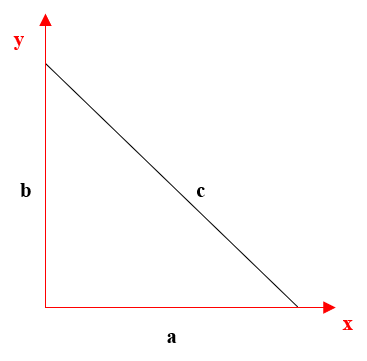
\includegraphics{{slides/coordaxes}}
\end{center}

\section{Generating Uniformly Distributed Random Points and angle}
\subsection{Points}
We initially tried generating the random points in a triangle just by finding random points in the x-y plane
\begin{verbatim}
  x = random.uniform(0,a)
  y = random.uniform(0,b)
\end{verbatim}

However we see that this does not work because the point may lie outside the triangle. So we use basic trignometery to see that $maxY = \frac{b(a-x)}{a}$ so we generate x the same as before but now limit y to this value like so
\begin{verbatim}
  x = random.uniform(0,a)
  maxY = (b(a-x))/a
  y = random.uniform(0,maxY)
\end{verbatim}
So we have the points inside the triangle but now there is another problem. The points in this triangle are not truly uniformly distributed which causes anamalous behaviour. This is because our $y$-value is dependent on the value of $x$ which meant that a higher percentage of our points ended up in the bottom half of the triangle.

To fix the issue we thought about the triangle as a rectangle with sides $a$ and $b$ and diagonal $c$. To generate uniformly distributed points for a rectangle, we can generate a random number between $0$ and $1$ and then multiply by $a$ to get the $x$-coordinate. Then to get the $y$-coordinate we generate another random number between $0$ and $1$ and then multiply by $b$. This doesn't work for our triangle as roughly half of the points would end up lying outside our triangle. To fix this issue, we reject any points that lie outside of our triangle; in other words we only accept the two random numbers generated if their sum is less than or equal to $1$. This then gives us uniformly distributed points within our triangle.

 To understand why this works we can consider vectors. Let $\mathbf{a}$ be a vector in the $i$ direction and let $\mathbf{b}$ be a vector in the $j$ direction. The magnitude of the vectors are determined by two different independent random numbers, $r_{1}$ and $r_{2}$ respectively (using rand.uniform). Both take values between $0$ and $1$. Thus the magnitude of $a$ is between $0$ and $a$ and the magnitude of b is between $0$ and $b$. All possible combinations of these vectors (since they are perpendicular and form a right angle) gives us a rectangle. The four vertices of our rectangle are formed by vectors $0i + 0j$, $\mathbf{a}i + 0j$, $0i + \mathbf{b}j$, $\mathbf{a}i + \mathbf{b}j$. Our triangle is formed by the three vertices: $0i + 0j$, $\mathbf{a}i + 0j$, $0i + \mathbf{b}j$.

 \begin{center}
   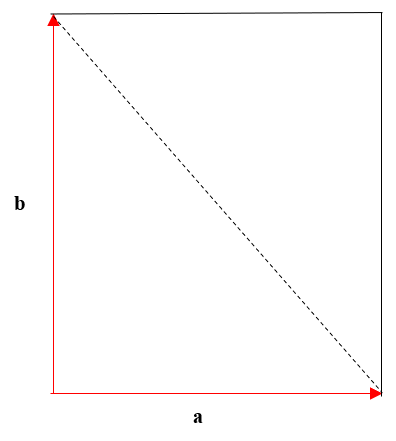
\includegraphics{{slides/vectorRect}}
 \end{center}

 To achieve points only within our triangle, the sum of our vectors must lie within the triangle. It is best to see this by considering the geometry/symmetry of the rectangle defined by the vectors. The dashed-line cuts our rectangle in half exactly and this line can be precisely reached from the origin by the vectors $r_{1} \mathbf{a} + r_{2} \mathbf{b}$ where $r_{1} + r_{2} = 1$.

Therefore, for the vector sum to lie in our triangle we require $r_{1} + r_{2} \leq 1$  i.e. this guarantees that our points are uniformly distributed only inside our triangle.

\subsection{Angle}
Generating a random angle is \emph{trivial}. We simply choose a random value between $0$ and $2\pi$ using rand.uniform

\section{Finding the probability}
\subsection{Equation of ant}
To find the probability we consider the path of of the ant in a straight line equation given a random point ( $(x_{0},y_{0})$) and angle($\theta$). We recall the equation
\begin{equation*}
  y = mx + c
\end{equation*}
We first determine the gradient $m$. consider the \emph{tangent} of $\theta$, we see that for the ant
\begin{equation*}
  tan(\theta) = \frac{\Delta y}{\Delta x}
\end{equation*}
So $tan(\theta) = m$ Now we need to determine $c$
\begin{align*}
  y &= mx+c \\
   &\implies c = y - mx \\
   &\implies c = y_{0} - tan(\theta) \cdot x_{0}
\end{align*}
So the path of the ant can be modelled by the straight line equation
\begin{align*}
  y = tan(\theta) \cdot x + (y_{0} - tan(\theta) \cdot x_{0})
\end{align*}
in the code $m$ is the antGradient and $c$ is the bIntercept. We also find the intercept with the $x$ axis as it may prove to be of use. So to to this we solve for $y=0$ i.e.
\begin{align*}
  0 &= tan(\theta) \cdot x + (y_{0} - tan(\theta) \cdot x_{0}) \\
    &= antGradient \cdot x + bIntercept \\
    &\implies x = -\frac{bIntercept}{antGradient}
\end{align*}
This value of $x$ will be called the aIntersect

\subsection{Quads}
Ok now that we have done this we have to decide which side the ant goes to. We imagine the ant's direction to be split into four quadrants i.e. ``quad" in the code. Then for each side we follow the instructions given and set the aCounter, bCounter and cCounter to $0$

\begin{center}
  \includegraphics{{quads}}
\end{center}
Now examine each each of the 4 cases invdividually
\subsubsection{Quad1}
\begin{center}
  \includegraphics{{quad1}}
\end{center}
Quad1 is defined for the values $ 0 \leq \theta \leq \frac{\pi}{2}$. When we have the ant pointing in this direction we can trivially see that no matter where the ant is it would always go to the side c. We do not need to check anything else and may increase the cCounter by $1$
\subsubsection{Quad2}
\begin{center}
  \includegraphics{{quad2}}
\end{center}
Quad2 is defined for the values $ \frac{\pi}{2} \leq \theta \leq \pi$. Now here we see that we need to do more work. There are two possible intersections either with $c$ or with $a$ as the diagram above shows that are possible.

In this Quad we are particularly interested in aIntersect. That is when we solve for given the equation of the ants path in this direction we can have  aIntersect $< a$ or  aIntersect $> a$.

\begin{center}
  \includegraphics{{quad2Intersects}}
\end{center}
In the diagram above the upper marker shows when aIntersect $> a$ and the lower marker shows when aIntersect $< a$. We conclude that in the case aIntersect $< a$ intersection is with side $a$ and we increase aCounter otherwise we increase cCounter.

\subsubsection{Quad3}
\begin{center}
  \includegraphics{{quad3}}
\end{center}
Quad3 is defined for the values $ \pi \leq \theta \leq \frac{3\pi}{2}$. There are two possible intersections either with $a$ or with $b$ as the diagram above shows that are possible. In this Quad we are again interested in aIntersect. Now we observe the following diagram
\begin{center}
  \includegraphics{{quad3Intersects}}
\end{center}
In the diagram above the upper marker shows when aIntersect $< 0$ and the lower marker shows when aIntersect $> 0$. We conclude that in the case aIntersect $< 0$ intersection is with side $b$ and we increase bCounter otherwise we increase aCounter.

\subsubsection{Quad4}
\begin{center}
  \includegraphics{{quad4}}
\end{center}
Quad4 is defined for the values $ \frac{3\pi}{2} \leq \theta \leq 2\pi$. There are two possible intersections either eith side $b$ or with $c$ as the diagram above shows that are possible. In this Quad we are now interested in the bIntercept. Now observe the following diagram
\begin{center}
  \includegraphics{{quad4Intersects}}
\end{center}
In the diagram above the upper marker shows when bIntercept $> b$ and the lower marker shows when bIntercept $< b$. We conclude that in the case bIntercept $< b$ intersection is with side $b$ and we increase bCounter otherwise we increase cCounter.

\subsection{Using the results}
Now that we have values for aCounter, bCounter and cCounter we simply divide each one by $N$ this gives us the exit probabilities as required.

\section{Lowest and Highest probabilities}
As we calculate the exit probabilities for each triangle we store the probability and array into a dictionary that takes the format
\begin{verbatim}
                            {probability : array}
\end{verbatim}
The reason for this is that we can then sort the dictionary by key value and place the probabilties in another array. The first value in this sorted probability array will always contain the smallest probability and the last value will always contain the largest probability. By doing it like this we have a one to one mapping of probability $\to$ array so we can simply get the array by looking up the dictionary value that had the key of the probability.
\end{document}
